\documentclass[final]{beamer}
\usepackage[size=custom,width=48,height=44,scale=0.78]{beamerposter}

\usepackage[T1]{fontenc}
\usepackage[utf8]{inputenc}
\usepackage{amsmath,amssymb,amsfonts,mathtools}
\usepackage{booktabs}
\usepackage{array}
\usepackage{graphicx}
\usepackage{ragged2e}

\setbeamertemplate{navigation symbols}{}
\setbeamertemplate{caption}[numbered]
\setlength{\abovecaptionskip}{0.4em}
\setlength{\belowcaptionskip}{0.2em}

\definecolor{cdaNavy}{RGB}{25,52,88}
\definecolor{cdaTeal}{RGB}{30,127,140}
\definecolor{cdaGold}{RGB}{197,146,55}
\definecolor{cdaLight}{RGB}{244,247,250}
\definecolor{cdaSoft}{RGB}{231,239,243}

\setbeamercolor{background canvas}{bg=white}
\setbeamercolor{normal text}{fg=black,bg=white}
\setbeamercolor{title}{fg=white,bg=cdaNavy}
\setbeamercolor{author}{fg=white,bg=cdaNavy}
\setbeamercolor{institute}{fg=white,bg=cdaNavy}
\setbeamercolor{block title}{fg=white,bg=cdaNavy}
\setbeamercolor{block body}{fg=black,bg=cdaLight}
\setbeamercolor{alertblock title}{fg=white,bg=cdaTeal}
\setbeamercolor{alertblock body}{fg=black,bg=cdaSoft}
\setbeamercolor{item}{fg=cdaTeal}

\setbeamertemplate{block begin}{
  \vskip1ex
  \begin{beamercolorbox}[colsep*=0.75ex,dp=1ex,center,rounded=true,shadow=true]{block title}
    \usebeamerfont{block title}\insertblocktitle
  \end{beamercolorbox}
  {\parskip0pt\par}
  \ifbeamercolorempty[bg]{block body}{}{\nointerlineskip\vskip-0.5pt}
  \usebeamerfont{block body}
  \begin{beamercolorbox}[colsep*=0.75ex,vmode,rounded=true,shadow=true]{block body}
}
\setbeamertemplate{block end}{
  \end{beamercolorbox}
}

\setbeamertemplate{alertblock begin}{
  \vskip1ex
  \begin{beamercolorbox}[colsep*=0.75ex,dp=1ex,center,rounded=true,shadow=true]{alertblock title}
    \usebeamerfont{block title}\insertblocktitle
  \end{beamercolorbox}
  {\parskip0pt\par}
  \ifbeamercolorempty[bg]{alertblock body}{}{\nointerlineskip\vskip-0.5pt}
  \usebeamerfont{block body}
  \begin{beamercolorbox}[colsep*=0.75ex,vmode,rounded=true,shadow=true]{alertblock body}
}
\setbeamertemplate{alertblock end}{
  \end{beamercolorbox}
}

\newcommand{\RR}{\mathbb{R}}
\newcommand{\cA}{\mathcal{A}}
\newcommand{\cB}{\mathcal{B}}
\newcommand{\simplex}{\Delta}
\newcommand{\one}{\mathbf{1}}
\newcommand{\norm}[1]{\left\lVert #1 \right\rVert}
\newcommand{\inner}[2]{\left\langle #1, #2 \right\rangle}
\newcommand{\paren}[1]{\left( #1 \right)}
\newcommand{\braces}[1]{\left\{ #1 \right\}}
\newcommand{\KL}{\mathrm{KL}}
\newcommand{\data}[1]{\textsc{#1}}
\newcommand{\ood}{\mathrm{OOD}}
\newcommand{\vsc}{\textsc{VSC}}
\newcommand{\bd}{\textsc{CDA-BD}}
\newcommand{\cda}{\textsc{CDA}}
\newcommand{\swad}{\textsc{SWAD}}
\newcommand{\diwa}{\textsc{DiWA}}
\newcommand{\eoa}{\textsc{EoA}}
\newcommand{\thetaw}{\bar{\theta}(w)}
\newcommand{\ub}{u_E}
\newcommand{\sourceflat}{\mathcal{F}^{\mathrm{src}}_\gamma}
\newcommand{\mixflat}{\mathcal{F}^{\mathrm{mix}}_\gamma}

\title{\vspace{0.2em}CDA: Post-hoc Domain Generalization by Distributional Canalization\vspace{0.1em}}
\author{Jayden Jeong \and Vijayan K. Asari}
\institute{Math, Science, and Technology Center (MSTC), Paul Laurence Dunbar High School \and School of Engineering, University of Dayton}
\date{}

\begin{document}
\begin{frame}[t]
\begin{columns}[t,totalwidth=\textwidth]

\begin{column}{0.32\textwidth}

\begin{block}{Introduction}
\small
Post-hoc domain generalization (\textbf{PDG}) methods deploy a final model \emph{after} training using only source-domain information collected from an existing checkpoint bank. This makes PDG attractive in practice: the base model does not need to be retrained from scratch just to test a new deployment rule.

\vspace{0.4em}
Strong PDG methods such as \swad{} and \diwa{} already show that checkpoint averaging can be highly effective under DomainBed-style evaluation. But they primarily select deployments from \emph{aggregate} signals:
\begin{itemize}
    \item \swad{} emphasizes \textbf{flatness} and overfit-aware averaging.
    \item \diwa{} emphasizes \textbf{diversity} across independently trained yet mergeable models.
\end{itemize}

\vspace{0.2em}
The new paper narrative is narrower and cleaner:
\begin{itemize}
    \item Aggregate source loss can hide which source domains are fragile.
    \item Diversity only helps when per-domain responses cancel in the right directions.
    \item \textbf{CDA therefore uses source-domain response geometry directly.}
\end{itemize}

\vspace{0.5em}
\centering
\fbox{\parbox{0.94\linewidth}{\centering\small\textbf{Core poster claim:} \cda{} selects and weights checkpoint soups using stability of \emph{per-domain losses} under source-mixture shift, not just flatness or diversity alone.}}
\end{block}

\begin{alertblock}{Theoretical Motivation}
\small
\textbf{Hidden-shift model.} Let the source-domain loss vector be
\[
L(\theta)=\paren{L_1(\theta),\dots,L_E(\theta)}^\top \in \RR^E,
\qquad
\bar L(\theta)=\frac{1}{E}\one^\top L(\theta).
\]
Assume the unseen target behaves like a nearby redistribution of source-domain mass:
\[
L_T(\theta) \le \alpha_T^\top L(\theta) + \epsilon_{\rm app},
\qquad
\cA_\rho = \braces{\ub + \delta : \one^\top\delta = 0,\ \norm{\delta}_2 \le \rho }.
\]

\textbf{CDA target-risk certificate.}
\[
L_T(\theta)
\le
\bar L(\theta) + \rho \norm{P_\perp L(\theta)}_2 + \epsilon_{\rm app}.
\]

\textbf{Exact robust source risk.}
\[
\sup_{\alpha \in \cA_\rho}\alpha^\top L(\theta)
=
\bar L(\theta)+\rho \norm{P_\perp L(\theta)}_2.
\]

So \(\bar L(\theta)\) alone is not enough. A model can have a low average source loss while remaining highly sensitive to source-mixture reweighting.

\vspace{0.4em}
\textbf{Why diversity is only useful directionally.} For retained checkpoints with centered responses \(c_j=P_\perp r_j\),
\[
\norm{P_\perp z(w)}_2^2
=
\sum_{j=1}^k w_j^2\norm{c_j}_2^2
2\sum_{1\le i<j\le k} w_i w_j \inner{c_i}{c_j}.
\]
Diversity helps only when the cross terms \(\inner{c_i}{c_j}\) \emph{cancel} hidden-shift sensitivity.
\end{alertblock}

\end{column}

\begin{column}{0.34\textwidth}

\begin{block}{CDA Algorithm / Implementation}
\small
\textbf{Input.} A completed checkpoint bank
\[
\cB=\braces{\theta_1,\dots,\theta_K}.
\]
\textbf{Output.} One deployed soup \(\thetaw\) together with source-side diagnostics.

\begin{center}
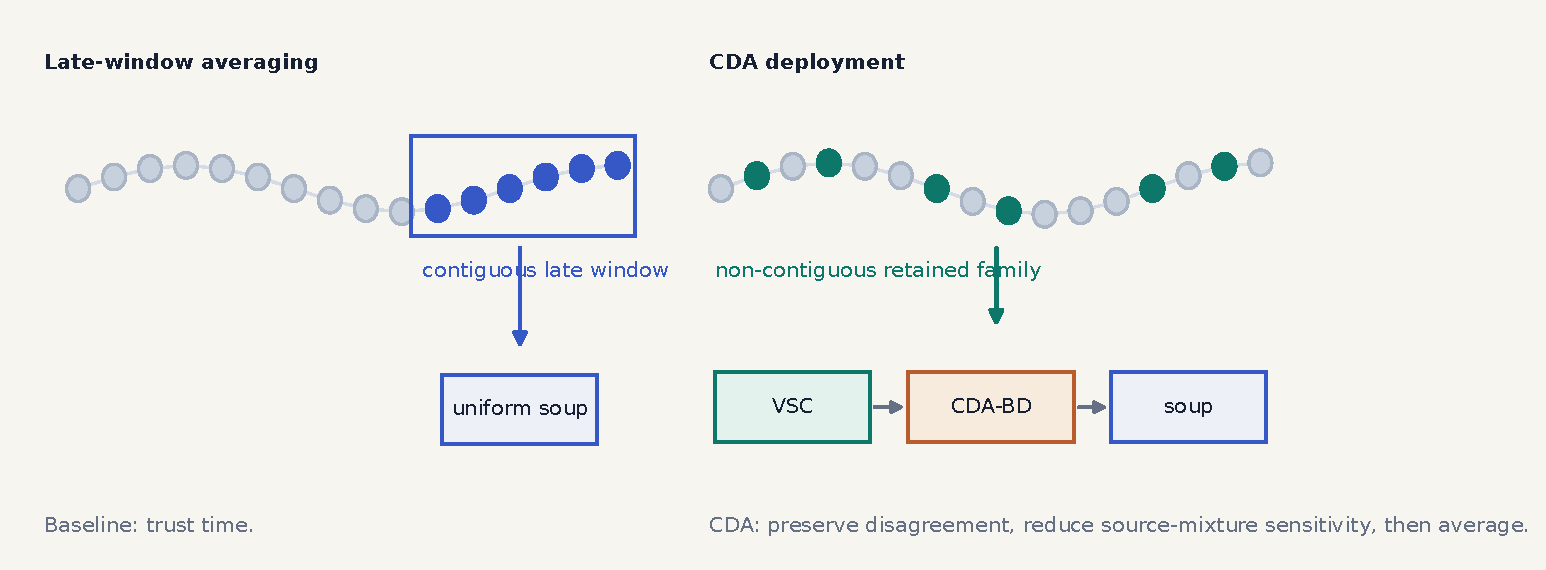
\includegraphics[width=0.90\linewidth]{figures/cda_sampling_overview.pdf}
\end{center}

\textbf{Step 1: Version Space Compression (\vsc{})}

For each source-support example \((x_i,y_i)\), let \(q_{j,i}=p_{\theta_j}(y_i\mid x_i)\). Define the full-bank disagreement mask
\[
D_\cB(i;\gamma)
=
\mathbf{1}\braces{
\exists j: q_{j,i}\ge \gamma
\ \text{and}\
\exists j': q_{j',i}<\gamma }.
\]
For a retained subset \(S\subseteq\cB\), the mismatch is
\[
d_{\rm vsc}(S,\cB;\gamma)
=
\frac{1}{m}\sum_{i=1}^m
\mathbf{1}\braces{D_S(i;\gamma)\ne D_\cB(i;\gamma)}.
\]
\vsc{} greedily retains a \emph{non-contiguous} family that preserves the checkpoint bank's informative disagreement structure on source data.

\vspace{0.5em}
\textbf{Step 2: Nonuniform weighting with \bd{}}

Let \(R\in\RR^{E\times k}\) collect the retained family source-loss vectors and define the coordinatewise best target
\[
b_e=\min_{1\le j\le k} R_{e,j}.
\]
\bd{} chooses \(w\in\simplex^k\) by solving
\[
\min_{w\in\simplex^k}
\frac{1}{E}\norm{Rw-b}_2^2
\lambda_{\rm ent}\KL(w\|u).
\]
The deployed soup is
\[
\thetaw=\sum_{j=1}^k w_j\theta_j.
\]

\vspace{0.5em}
\textbf{Deployment bridge.} The retained-family certificate for the final soup is
\[
L_T(\thetaw)
\le
\bar z(w)
\rho\norm{P_\perp z(w)}_2
\paren{E^{-1/2}+\rho}M(w)
\epsilon_{\rm app},
\]
where \(z(w)=\sum_j w_jL(\theta_j)\) and \(M(w)=\norm{L(\thetaw)-z(w)}_2\) is the \emph{mergeability remainder}.

\end{block}

\end{column}

\begin{column}{0.34\textwidth}

\begin{block}{Results}
\small
\textbf{Headline benchmark result.} On the five DomainBed benchmarks, \cda{} reaches the strongest reported average \(\ood\) accuracy in the comparison package.

\begin{center}
\renewcommand{\arraystretch}{1.18}
\begin{tabular}{lcccccc}
\toprule
\textbf{Method} & \textbf{PACS} & \textbf{VLCS} & \textbf{OH} & \textbf{TI} & \textbf{DN} & \textbf{Avg.}\\
\midrule
ERM & 85.5 & 77.5 & 66.5 & 46.1 & 40.9 & 63.3\\
\swad{} & 88.1 & 79.1 & 70.6 & 50.0 & 46.5 & 66.9\\
\diwa{} & 89.0 & 78.6 & 72.8 & 51.9 & 47.7 & 68.0\\
\cda{} & \textbf{89.1} & \textbf{79.5} & \textbf{72.9} & \textbf{52.3} & \textbf{47.8} & \textbf{68.3}\\
\bottomrule
\end{tabular}
\end{center}

\vspace{0.4em}
\begin{itemize}
    \item \cda{} improves over \swad{} by \(+1.4\) average points.
    \item \cda{} improves over \diwa{} by \(+0.3\) average points.
    \item \cda{} is the best row on \(4/5\) benchmark columns in this package.
\end{itemize}

\vspace{0.2em}
\textbf{Mechanism evidence.} The paper's diagnostic layer measures the certificate terms directly rather than only reporting final accuracy.

\begin{center}
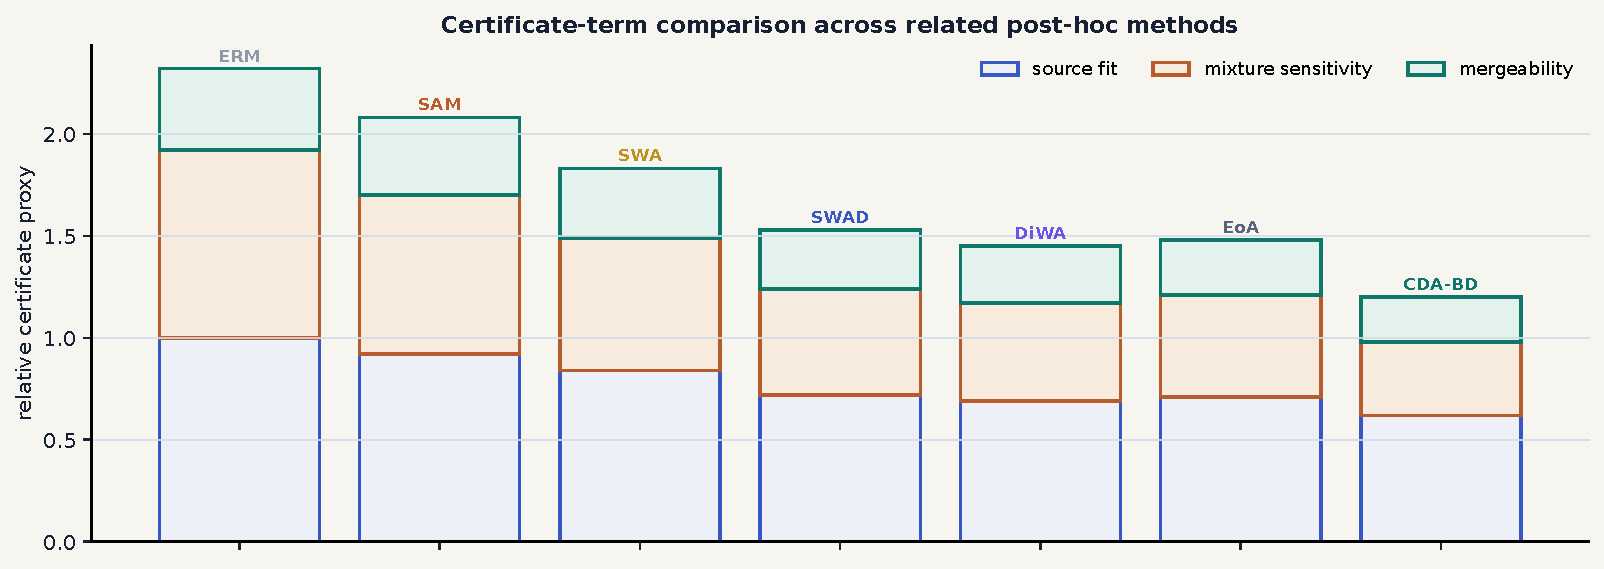
\includegraphics[width=0.86\linewidth]{figures/certificate_proxy_comparison.pdf}
\end{center}

\small
\textbf{Reading the diagnostic.} \swad{} mainly improves fit and mergeability through flatter deployment regions, \diwa{} reduces redundancy through diversity, and \cda{} is designed to reduce the \emph{centered source-mixture sensitivity} term most directly.
\end{block}

\begin{block}{Discussion}
\small
\textbf{Takeaways}
\begin{itemize}
    \item Post-hoc DG is a \textbf{deployment problem}: choose a checkpoint family and a weight vector from source-only evidence.
    \item Flatness and diversity remain useful, but they are not the final deployment objective in CDA.
    \item \cda{} reframes checkpoint averaging around \textbf{distributional canalization}, i.e. stability of per-domain losses under source-mixture perturbations.
\end{itemize}

\textbf{Limitations}
\begin{itemize}
    \item The theory assumes a \textbf{local source-supported hidden shift}. If the target is not well approximated by nearby source-mixture redistributions, the certificate can become loose.
    \item The margin over \diwa{} is \textbf{modest}. The main claim is not universal dominance; it is that a source-aware certificate yields a competitive and more interpretable deployment rule.
\end{itemize}
\textbf{Selected references.} \scriptsize
[1] Gulrajani and Lopez-Paz, \emph{In Search of Lost Domain Generalization}, ICLR 2021.\par
[2] Cha et al., \emph{Domain Generalization by Stochastic Weight Averaging Densely}, NeurIPS 2021.\par
[3] Ram\'e et al., \emph{Diverse Weight Averaging for Out-of-Distribution Generalization}, NeurIPS 2022.\par
[4] Arpit et al., \emph{Ensemble of Averages}, NeurIPS 2022.
\end{block}

\end{column}

\end{columns}
\end{frame}
\end{document}
